\chapter{Introduction}

\todo{general intro}

\section{Proteins}
The central objects of study in this work are proteins. The complexity of proteins begs some explanation, which we provide here for the non-biologically oriented reader, who may not already be familiar with this topic.

Aside from this background, we do not further significantly concern ourselves with the biological particularities -- we are computer scientists, not biologists. For the same reason, we apologize for any errors or shortcomings of the following explanation.

\subsection{Function}
Proteins are large molecules (macromolecules) that are used by organisms in virtually every part of their function. For example, proteins are used as enzymes or hormones, to name just a few. However, proteins are also widely used in the biological industries for a variety of purposes, including medical purposes, food processing and biological detergents. These industries would benefit greatly from an increased understanding of proteins, as this would aid their efforts in protein engineering. Protein engineering is the process of developing and synthesizing proteins useful to the above-mentioned industries.

The usefulness of proteins cement the reasoning for their extensive study, including this work. Proteins are incredibly complicated, intricate biological machinery. A better understanding of their complex behavior and properties could lead to the development of better, more useful proteins, which could ultimately decrease suffering and/or save lives in the medical area or decrease costs and increase efficiency in the other biological industries.

%\subsection{Construction?}
\subsection{Structure}
Proteins are macromolecules, consisting of long chains of \textit{amino acids}. Amino acids are a class of organic compounds, of which about 20 are used in proteins. Proteins commonly consists of hundreds of amino acids, connected together in a sequence, making proteins molecules of potentially thousands of atoms. In nature, proteins are constructed by organisms by reading their genetic code, in the form of DNA. The genetic code (genes) of the DNA describes which amino acids to put together in a sequence, in order to construct the desired protein.

A protein is in theory defined entirely by its amino acid sequence. However, when proteins are assembled, the chain of amino acids folds up into a complex 3-dimensional structure. This structure is what largely determines the function and properties of the protein. When speaking of protein structure, we concern ourselves with three main levels of structure:

\begin{description}
    \item[Primary Structure:] Purely the 1-dimensional amino acid sequence itself, with no additional information about the 3-dimensional structure of the protein.
    \item[Secondary Structure:] 3-dimensional structure of local parts of the protein. When folding, local parts of the amino acid sequence arranges itself into certain structures, most commonly \textit{$\alpha$-helices} and \textit{$\beta$-sheets}. Secondary structure is knowledge of each amino acid's type of local structure.
    \item[Tertiary Structure:] The full specification of the folded protein, that is, the 3-dimensional coordinates of all the amino acids.
\end{description}

See figure \ref{fig:protein_structure} for an illustration of the three levels of protein structure.

\begin{figure}
    \centering
    \includegraphics[width = \linewidth]{report/figures/protein_structure.png}
    \caption{Depiction of the levels of protein structure -- primary, secondary and tertiary. \cite{protein_structure_fig}}
    \label{fig:protein_structure}
\end{figure}

A central task in protein machine learning is prediction of secondary or tertiary structure, given the primary structure. Many models have some success when predicting secondary structure, as it is not a very difficult task. Comparatively, predicting tertiary structure from primary structure alone is an incredibly difficult task, as the folding of a protein is such a complicated process.

In this work, we concern ourselves with prediction of various protein properties (including secondary structure, but not tertiary structure), given only the protein's primary structure. In doing this, we consider the protein's primary structure as merely a sequence of the common amino acids. Since there are not that many, each amino acid can be assigned a letter of the alphabet, resulting in a protein being represented as merely a string of letters (for example, ``MSKG...'' \todo{insert some letters from actual protein here}).

\subsection{Relation to Natural Language Processing}
With the above format of the protein data in mind, the similarity between protein machine learning and natural language processing (NLP) becomes apparent. In NLP, the data is in the form of written text, most commonly represented as a sequence of words. We can view our protein data as a similar sequence, except that the words of proteins are amino acids, and while natural languages has hundreds of thousands of words, proteins have just 20 amino acids. Proteins can be thousands of amino acids long, and similarly, documents may be thousands (if not tens or hundreds of thousands) words long. It is clear that, despite some differences, the fields of NLP and protein machine learning are related.

With this relation in mind, we should look to NLP for inspiration for methods in machine learning to apply to proteins. As it turns out, many of the ideas in NLP can also be used in protein machine learning.

\section{Deep Learning}


\section{Related Work}

% the problem (description)
% current state of the art - problems and status
% two problems: ...

% (1) no direct generative process, no interpolations with current methods (unirep)
% (2) it is not a probabilistic model; Uncertainty is not accounted for

% without a probabilistic model, the representation cannot actively be used as a

% our project

% why we chose to be two working on the project.

% Why is this interesting for NN and NZ:

% proteins based drugs.
% peptider mutationer

% This is fine for your MSc project. For the Novo grant, we will need to spice it up a bit, adding some comments about ultimately impact etc.

% The structure of such applications is typically in the form of:
% 1. What is the problem. E.g "Understanding how mutations in amino acid sequences affect protein structure and function is a central challenge in computational biology, ..."
% 2. What are the limitations/problems with current state-of-the-art solutions to this problem. E.g., "recently important progress has been made in this area using representation-learning techniques, which have... However, current approaches have extracted such representations, as the internal state of... This makes it difficult to incorporate notions of uncertainty, and other essential properties that we would normally impose on representations. ... In addition, current approaches are not generative, in the sense that we cannot generate protein sequences corresponding to any point in latent space. "
% 3. What will you do. "In this project, we will investigate the possibility of learning
% 4. How will this improve the world.

\section*{Background}
Understanding how mutations in amino acid sequences affect protein structure and function is a central challenge in computational biology. Machine learning has proven to be a useful tool in the analysis of protein sequences. One form of machine learning that has been effectively applied to this problem is \textbf{representation learning}.

Representation learning is the task of training a machine to produce a suitable representation of features for the desired input, as opposed to manually engineering the representation. Good representations are important in order to learn useful properties of the given data.

Previous attempts at \textbf{protein sequence learning} have shown that fundamental structural features, that capture the function of a given protein, can be learned and represented from raw protein sequences by using Deep learning \cite{alley2019unified}. Specifically, using a \textbf{recurrent neural network} to summarize any protein sequence into a fixed length vector and subsequently averaging, such statistical representations can be discerned from large sets of input data. Additionally, such approaches have been shown to improve performance in nearly all models on downstream tasks \cite{rao2019evaluating}.

Protein sequences are \textbf{comparable to natural language sentences}: both consists of a sequence of symbols. Sentences consists of the letters of the alphabet, while proteins are amino acids. Thus one might look at the results of natural language sentence representations in order to learn about protein sequence representation. A study by Google Brain \cite{bowman2015generating} showed that one can represent entire sentences as single vectors in a \textbf{latent space}, allowing interpolation between sentences. Additionally, the latent space inherently maps common properties of sentences, such as style and topic. It is possible that a similar representation for proteins may be able to \textbf{map properties of proteins, such as secondary structure}.

\textbf{Unsupervised learning} is particularly suited for protein machine learning, since there is an overweight of unlabeled data. If a powerful unsupervised model could be produced, the wealth of this data could be used effectively \cite{AlQuraishiUnsupervised}. Therefore, unsupervised or variants like semi- or self-supervised learning methods could be useful.

Unsupervised representation learning has recently been applied to protein sequences \cite{alley2019unified} in order to achieve a latent space representation. However, current approaches have extracted such representations, as the hidden internal state of a recurrent layer in the learning network. This makes it difficult to incorporate notions of uncertainty, and other essential properties that we would normally impose on such representations. That is, current approaches are not generative, and so we cannot generate protein sequences corresponding to any point in latent space.

Current work on representations of proteins might carry potential toward a \textbf{general representation of proteins}, implying that general unseen protein sequences can be analyzed with such a representation with respect to functionality or structure, or at least infer commonalities from their representations. We wish to explore such implications.

\section*{Aims and Method}
This project revolves around applying representation learning to protein sequences. We wish to examine the performance of representations and their implications for protein informatics, by developing an unsupervised representation of protein sequences, using tools from machine learning such as variational autoencoders and deep neural networks. The results will be compared with current state-of-the-art.

Initially, we wish to inspect the unsupervised UniRep model \cite{alley2019unified} which compresses protein sequences into a fixed length vector, representing the sequence in a latent space. One key aspect is that the representations created by UniRep corresponds to the internal state of the LSTM used for training. In this project, we wish to make a proper representation instead, meaning that the representation itself is the output, not the internal state. The hope is that such a model would produce an overall better representation, with better performance on standard benchmarks.

The latent space defined by such a representation might allow for an understanding of protein sequences, by defining a mapping from sequences to protein properties, such that similar proteins are close together in the space (see figure \ref{fig:latentSpace}). Previously unseen points could correspond to unseen protein sequences, and properties of these proteins could be inferred from the latent space.

In addition, it will be useful to use representations to explain the behavior of variants of protein that we know, but we need to optimize. For example, the representation is important to help explaining the experimental results of variants screening, trying to map the effect of mutations, especially in case when we do not have a structure.

\begin{figure}[ht]
    \centering
    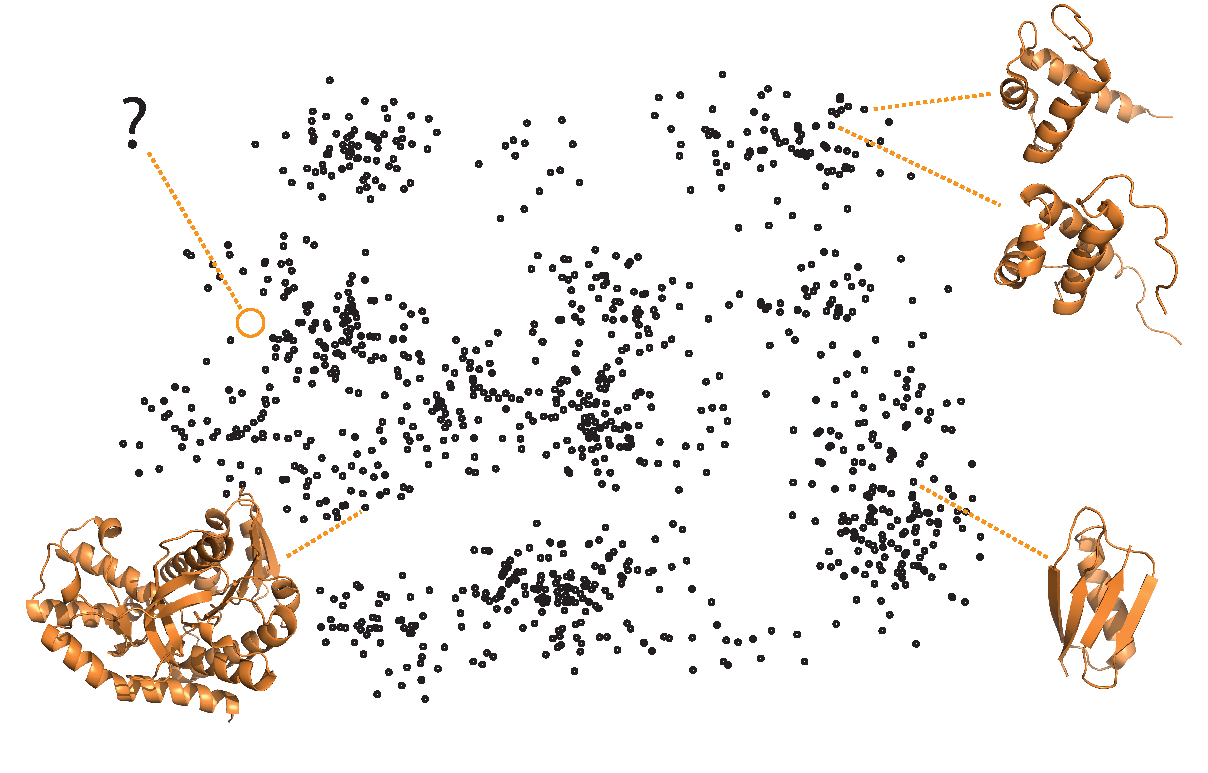
\includegraphics[width=\textwidth]{figures/figure.pdf}
    \caption{A 2-dimensional view of a protein sequence representation. Similar proteins have representations that are close together. With such a representation, small changes in protein can be explored in the space by looking at points close to the protein. Properties of unknown sequences (represented here by the question mark) could potentially be explored by examining the representation space.}
    \label{fig:latentSpace}
\end{figure}

% \section*{Project Plan}
% We will start by identifying strengths and weaknesses in current state-of-the-art techniques. This would give us a solid foundation on which to build our new model.

% We wish to examine which types of neural networks best suit the learning task, by exploring both convolutional neural networks (CNNs) and recurrent neural networks (RNNs).

% Then we assess the quality of different types of representations, such as those achieved by considering the entire sequence at once versus representations as a combination of sub-representations of the sequence's components.

% Finally, to evaluate the project aims, we will compare the results with the current state-of-the-art. Table \ref{schedule} shows a proposed schedule for the project.

% \begin{center}
% \begin{table}[H]
% \begin{tabular}{lclll}
% \textbf{Project Plan} & \textbf{Schedule (months)}        &  &  &  \\ \cline{1-2}
% \multicolumn{1}{|l|}{\begin{tabular}[c]{@{}l@{}}Preliminaries: \\ Identify strengths and weaknesses on current state-of-the-art\end{tabular}}                         & \multicolumn{1}{c|}{1}   &  &  &  \\ \cline{1-2}
% \multicolumn{1}{|l|}{\begin{tabular}[c]{@{}l@{}}Modelling: \\ Recurrent vs Convolutional Neural Networks\end{tabular}}                                                     & \multicolumn{1}{c|}{1-3} &  &  &  \\ \cline{1-2}
% \multicolumn{1}{|l|}{\begin{tabular}[c]{@{}l@{}}Latent space structuring: \\ Entire sequence representation vs. position representation and transitions\end{tabular}} & \multicolumn{1}{c|}{3-5} &  &  &  \\ \cline{1-2}
% \multicolumn{1}{|l|}{\begin{tabular}[c]{@{}l@{}}Applications: \\ Performance of results in comparison with current-state-of-the-art\end{tabular}}                     & \multicolumn{1}{c|}{6}   &  &  &  \\ \cline{1-2}
% \end{tabular}
% \end{table}
% \label{schedule}
% \end{center}

% \section*{Feasibility}
% This project is ambitious, but we both have strong backgrounds in computer science, with bachelor degrees with very high average grades. We finished our bachelor degrees with a project within the field of machine learning as well, and wish to repeat the success. During our master's degree we have taken multiple elective courses in machine learning, which will be invaluable to this project.

% We chose to work as a group because of two factors: the project scope and its length. While the project is ambitious, we only have 6 months to complete it. A single student would likely not be able to achieve this. Please note that because of the duration of the project, funding both of us through the scholarship amounts to the same expense as supporting a single student for a longer project of 12 months, which is common in other university departments.

% The project will be supervised by Wouter Krogh Boomsma, who specializes in machine learning methods for biomolecular data at the Department of Computer Science, University of Copenhagen, which provides an ideal setting for the execution of this project.

% Wouter has existing collaborations to Novozymes (Lars Olsen, Protein Engineering), on the task of protein stability prediction. One of the ideas behind the current MSc project was to establish closer ties to protein research at Novo Nordisk, through this collaboration with Research Scientist Daniele Granata, in the Modelling and Predictive Technologies Department.

% \section*{Interest to Novo Nordisk and Novozymes}
% The application of protein sequence representations could be immense within analysis and understanding of new proteins and their function, especially when detailed structural information is not easily available. Importantly, the approach will give the opportunity to build tailored sequence models for specific classes of compounds of interest for Novo Nordisk and Novozymes, for example antibodies, nanobodies, or peptides libraries.

% Obtaining an accurate representation of protein sequences can represent a fundamental tool for interpreting and rationalizing the results of experimental screenings, enabling also the exploitation of other machine learning approaches toward the automatized generation of new variants.

% These ideas greatly agree with the recent efforts of Novo Nordisk to enlarge the exploitation of Data Science and AI technologies in its drug discovery process. We have no doubt that Novozymes could benefit from this technology as well.

% In addition, this field of research, being the understanding and formulation of protein sequence space, is comparatively new, allowing for many different ventures to be explored. This project is one step in that direction.

% I suggest that the goal of the main project should be that we try to create a proper representation, rather than simply using the internal state of the LSTM. We will do this by using variational auto encoders. The challenge here is that we need to encode *sequences* of inputs.

% Daniele
% Protein sequence models would be a great subject actually. Regarding the application, it seems pretty simple and it requires very little information in general and also for the project (Description of project in English, maximum 1,200 words. Please include background, aim and project plan and how this project is of interest to Novo Nordisk) especially if you have already proposals around.

% Wouter
% Unified rational protein engineering with sequence-only deep representation learning
% This is the first (or one of the first) applications of using language models to learn representations of protein sequences.
% https://www.biorxiv.org/content/10.1101/589333v1
% One of the authors, Mohammed Alquraishi (a collaborator of ours), also writes some of his thoughts on the method on his blog: https://moalquraishi.wordpress.com/2019/04/01/the-future-of-protein-science-will-not-be-supervised

% Evaluating Protein Transfer Learning with TAPE
% This is a very recent manuscript (will probably be published at NeurIPS this year) about representation learning of biological sequences. It is interesting because it asks the question how much different downstream tasks can be improved by first learning a good representation - and they present a benchmark set that is likely to become standard in the field (which we might use in the project).

% In the preproject, I suggest we try and reproduce the results of the first article, but with CNNs instead of RNNs. I suggest that the goal of the main project should be that we try to create a proper representation, rather than simply using the internal state of the LSTM. We will do this by using variational auto encoders. The challenge here is that we need to encode *sequences* of inputs. Here is one of the first papers that tries to do encode/decode sequences of words: https://arxiv.org/abs/1511.06349. There are a some difficulties getting this to work, and some newer references that try to resolve this, but I think you have enough reading material for now :) Again, we will try to use CNNs in addition to LSTMs, to compare pros/cons of the two approaches.

% I do not expect you to have a full overview over this literature when we meet - so don’t stress too much if there are things you don’t understand in these papers. But it would be great if you could try to write the main points of your thesis project in your own words - so we have something to discuss when we meet on the 27th.
